% https://tex.stackexchange.com/a/466572
\documentclass{beamer}
\usepackage{verbatim}
\usepackage{caption,subcaption}
\newcommand{\noi}{\noindent}

\usepackage{tikz}
\usetikzlibrary{shapes.geometric}
\newcounter{Angle}

\setbeamersize{text margin left=1.15in,text margin right=1.15in}

\begin{document}

\begin{frame}
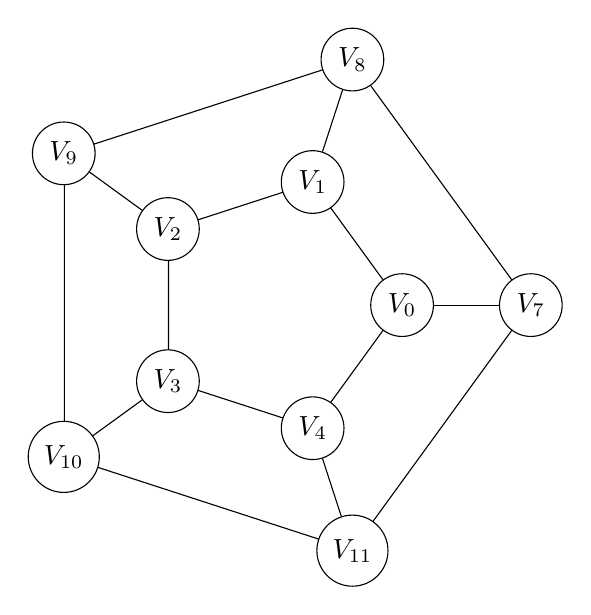
\begin{tikzpicture}[scale=0.55]
    \node[regular polygon,draw,regular polygon sides=5,minimum
    size=3.27cm,rotate=-90] (small 5gon){};
    \node[regular polygon,draw,regular polygon sides=5,minimum
    size=6.54cm,rotate=-90] (large 5gon){};
    \begin{scope}[every node/.append style={draw,shape=circle,fill=white}]
     \foreach \X [count=\Y starting from 0,evaluate=\Y as \Z using {int(\Y+1)}] in {7,...,11}
     {\node (v\Y) at (small 5gon.corner \Z){$V_\Y$};
     \node (v\X) at (large 5gon.corner \Z){$V_{\X}$};
     \draw (v\Y) -- (v\X);}
    \end{scope}
\end{tikzpicture}
\end{frame}
\end{document}
